\documentclass{sig-alternate-10pt}

\usepackage[l2tabu,orthodox]{nag}  % Check for use of obsolete LaTeX packages/constructs
\usepackage[utf8x]{inputenc}       % This file is formatted in UTF-8
\usepackage{upquote}               % Fix quotes in verbatim environments

\usepackage{graphicx}              %
\usepackage{amsmath}               % http://ctan.org/pkg/amsmath
%% this breaks tikz... badly...
%\usepackage[all]{onlyamsmath}      % http://ctan.org/tex-archive/macros/latex/contrib/onlyamsmath
\usepackage{url}                   % http://ctan.org/tex-archive/macros/latex/contrib/url
\usepackage[caption=false]{subfig} % http://ctan.org/tex-archive/macros/latex/contrib/subfig
                                   % The subfig package is deprecated in favour of subcaption,
                                   % but as of April 2015 subcaption doesn't work with ACM or
                                   % IEEE style files (this is also the reason for [caption=false])

\usepackage{verbatim, xcolor}
\usepackage{whix} %% shiny wcix diagrams
\usepackage{todonotes}
\newcommand{\narrative}[1]{\textcolor{blue}{(narrative: #1)}}

\begin{document}

% % Copyright
% \setcopyright{acmcopyright}
% %\setcopyright{acmlicensed}
% %\setcopyright{rightsretained}
% %\setcopyright{usgov}
% %\setcopyright{usgovmixed}
% %\setcopyright{cagov}
% %\setcopyright{cagovmixed}


% % DOI
% \doi{10.475/123_4}

% % ISBN
% \isbn{123-4567-24-567/08/06}

% % Conference
% \conferenceinfo{PLDI '13}{June 16--19, 2013, Seattle, WA, USA}

%\acmPrice{\$15.00}

%
% % --- Author Metadata here ---
% \conferenceinfo{WOODSTOCK}{'97 El Paso, Texas USA}
% %\CopyrightYear{2007} % Allows default copyright year (20XX) to be over-ridden - IF NEED BE.
% %\crdata{0-12345-67-8/90/01}  % Allows default copyright data (0-89791-88-6/97/05) to be over-ridden - IF NEED BE.
% % --- End of Author Metadata ---

\title{RemIX: A Distributed Internet Exchange for Networks in Remote Places
% \titlenote{(Produces the permission block, and
% copyright information). For use with
% SIG-ALTERNATE.CLS. Supported by ACM.}
}
% \subtitle{(Pronounced 'kicks,' for Community Internet Exchange)
% \titlenote{A full version of this paper is available as
% \textit{Author's Guide to Preparing ACM SIG Proceedings Using
% \LaTeX$2_\epsilon$\ and BibTeX} at
% \texttt{www.acm.org/eaddress.htm}}
%}

%
% You need the command \numberofauthors to handle the 'placement
% and alignment' of the authors beneath the title.
%
% For aesthetic reasons, we recommend 'three authors at a time'
% i.e. three 'name/affiliation blocks' be placed beneath the title.
%
% NOTE: You are NOT restricted in how many 'rows' of
% "name/affiliations" may appear. We just ask that you restrict
% the number of 'columns' to three.
%
% Because of the available 'opening page real-estate'
% we ask you to refrain from putting more than six authors
% (two rows with three columns) beneath the article title.
% More than six makes the first-page appear very cluttered indeed.
%
% Use the \alignauthor commands to handle the names
% and affiliations for an 'aesthetic maximum' of six authors.
% Add names, affiliations, addresses for
% the seventh etc. author(s) as the argument for the
% \additionalauthors command.
% These 'additional authors' will be output/set for you
% without further effort on your part as the last section in
% the body of your article BEFORE References or any Appendices.

\numberofauthors{6} %  in this sample file, there are a *total*
% of EIGHT authors. SIX appear on the 'first-page' (for formatting
% reasons) and the remaining two appear in the \additionalauthors section.
%
\author{
% You can go ahead and credit any number of authors here,
% e.g. one 'row of three' or two rows (consisting of one row of three
% and a second row of one, two or three).
%
% The command \alignauthor (no curly braces needed) should
% precede each author name, affiliation/snail-mail address and
% e-mail address. Additionally, tag each line of
% affiliation/address with \affaddr, and tag the
% e-mail address with \email.
%
% 1st. author
 \alignauthor
 William Waites \\ %\titlenote{Dr.~Trovato insisted his name be first.}\\
%        \affaddr{Institute for Clarity in Documentation}\\
%        \affaddr{1932 Wallamaloo Lane}\\
%        \affaddr{Wallamaloo, New Zealand}\\
%        \email{trovato@corporation.com}
% 2nd. author
 \alignauthor
 Roger Baig
 \alignauthor
 Peter Buneman \\ %\titlenote{The secretary disavows
% any knowledge of this author's actions.}\\
%        \affaddr{Institute for Clarity in Documentation}\\
%        \affaddr{P.O. Box 1212}\\
%        \affaddr{Dublin, Ohio 43017-6221}\\
%        \email{webmaster@marysville-ohio.com}
% % 3rd. author
\and
 \alignauthor
 Marwan Fayed \\ %\titlenote{This author is the
% one who did all the really hard work.}\\
%        \affaddr{The Th{\o}rv{\"a}ld Group}\\
%        \affaddr{1 Th{\o}rv{\"a}ld Circle}\\
%        \affaddr{Hekla, Iceland}\\
%        \email{larst@affiliation.org}
% use '\and' if you need 'another row' of author names
% % 4th. author
 \alignauthor
 Michael Fourman \\
%        \affaddr{Brookhaven Laboratories}\\
%        \affaddr{Brookhaven National Lab}\\
%        \affaddr{P.O. Box 5000}\\
%        \email{lleipuner@researchlabs.org}
\alignauthor
Richard Simmons \\
%        \affaddr{Brookhaven Laboratories}\\
%        \affaddr{Brookhaven National Lab}\\
%        \affaddr{P.O. Box 5000}\\
%        \email{lleipuner@researchlabs.org}
}


\maketitle
\begin{abstract}
Rural access networks are designed to bridge the `last-mile' broadband gap in regions that are under-served by traditional broadband providers. Their construction is bespoke, driven by their beneficiaries, and determined by physical landscape, population distribution, and monetary budget. Irrespective of their differences, they are joined by one substantial challenge: connecting to the rest of the Internet is prohibitively expensive. HUBS \textsc{c.i.c} was created in Scotland to respond to this. It is a co-operative of access network members that generates the economies of scale required to afford backhaul and Internet transit. While intermediation at the IP layer between the members and the Internet is required for reasons of scale, it is neither necessary nor desirable amongst the member networks themselves. In urban areas, networks could interconnect with each other at an Internet Exchange Point (IXP). In Scotland where the networks are scattered across 80,000km$^2$ of mountain, field, and sea it is not so easy. We bridge this gap with a design for a distributed Internet exchange for access networks in remote places. Doing so allows for bilateral arrangements for mutual support and assistance between these networks, and increases the resilience of access network connectivity. We present the relevant components, and describe our implementation, so that our efforts may be reproduced. 
\end{abstract}


%
% The code below should be generated by the tool at
% http://dl.acm.org/ccs.cfm
% Please copy and paste CCSXML code instead of the example below.
%

\section{Introduction} \label{sec:intro} In remote and rural regions the last-mile problem has been the subject of much
focus. Deployments in remote regions of the world have shown that it is possible
to build high quality access networks in otherwise under-serviced
regions~\cite{xxx}. Their underlying technologies range in medium (eg. copper
or fibre-optic cabling, licensed or unlicensed wireless), energy (eg. solar or
wind generation or mains supplied), and topology.
%(eg. multi-hop, one-to-many\narrative{not quite sure what these two %mean}).
Successful deployments, including our own in Scotland,
have two attributes in common:
\begin{inparaenum}[(i)]
  \item Networks designs are bespoke, suggesting
    there is no one-size-fits-all solution;
  \item crucially, communities must be invested and
    involved~\cite{Wallace:2015a,Wallace:2015b}.
\end{inparaenum}

Though remote access network research is far from complete, the next question is
increasingly clear: What options do remote, isolated networks have for
`backhaul' to interconnect with the rest of the Internet? We define ``remote''
as far from urban areas where commodified network infrastructure is available.
For example long-distance circuits, if and where they are available, are both
expensive and difficult to reach. Access networks in remote places serve
populations that are dispersed. The lower population density reduces the size of
their user-base when compared to their urban cousins. With no options for
interconnecting with nearby networks to generate economies of scale,
\emph{high-quality} backhaul is prohibitively expensive, if it exists at all.

% , almost by definition, and even in the best case such a network will usually
% not have enough of with a userbase  to the nearest city several hundred
% kilometers away\footnote{For example, the main case-study of this paper, a
% network on the West Coast of Scotland is 240km from the nearest major city that
% has datacentres and any diversity of network infrastructure to speak of.}.

The absence of resource pooling options for remote networks is the focus of this
paper. One such example is operated by the Guifi Foundation~\cite{guifi}. Guifi
operates a regional backbone network as a commons. The abstraction that is
presented to clients is an exchange point implemented over IP. In this type of
network, relationships between end-users are either mediated by Guifi, or
implemented as an overlay.

The \acf{IXP} is a long-standing structure that plays a pivotal role in
facilitating interconnections between networks~\cite{Ager:2012,Chatzis:2013}. We
are motivated by \acp{IXP} for two reasons. First, the primary role of an
\ac{IXP} is economic. Member networks can connect $n$ networks at an IXP with
$n$ circuits, rather than arranging for $\frac{n^2}{2}$ circuits independently.
Second, the \ac{IXP} model of multilateral public peering leads to high density
interconnections, and traffic across the exchange that can be comparable in
magnitude to the largest global service providers~\cite{Ager:2012}. Together,
they are an indication that such a topology might be used to improve
inter-connectivity between networks in under-serviced regions, and to pool
otherwise expensive backhaul resources.

In this paper we present RemIX, a \emph{distributed} Internet Exchange for
Remote and rural networks. The RemIX architecture is agnostic to underlying
technologies, embedding the same principles as the successful remote networks it
is designed to serve. It distinguishes itself from \acp{IXP} by the vast
distances permitted between points of presence, and the lower density of member
networks that connect to them. The trade-off between distance and density gives
rise to the idea of \emph{lightweight} points of presence. The lightweight
nature is advantageous, in that as few as two member networks are sufficient to
establish a point of presence. The RemIX switching fabric is agnostic to
physical layer technology and topology.

We describe our RemIX implementation in Scotland. In its current form our
deployment services a \~2000km$^2$ region that spans sea and mountainous
mainland. Implementation details are provided, with motivating rationale, so
that others may benefit from our efforts. Functionally, our implementation
appears to its members as a large Ethernet switch. Crucially, RemIX allows
member networks to establish unmediated relationships between themselves.

In the following sections we further motivate \acp{IXP} as an ideal model. We
then discuss the RemIX architecture in detail. Our deployment is then described,
along with lessons learned. Finally, a broader context of the local environment
is presented before concluding remarks.


\section{Community Network Environment} \label{sec:context} In this section we give a brief overview of \acp{IXP}, and then set the context for the local Scottish environment before summarizing our early efforts.

\subsection{Internet Exchange Points (IXPs)}

As part of the decommissioning of the \ac{NSFNET} in the early-mid 1990s, four
\acp{NAP} were created. They were operated by large American telephone companies
(MCI, Sprint, PacBell, Ameritech) and designed to prevent partitioning of the
commercial Internet~\cite{hayes1997computing,Ager:2012}. Their high costs and equipment requirements created barriers to participation.
\acp{IXP} emerged as an alternative, appearing in carrier-neutral facilities. Worldwide, \acp{IXP} now number in the hundreds.

Networks that connect via \ac{IXP} are free to make arrangements with any other network. Economic conflicts of interest are most often avoided by organizing the \ac{IXP} as a not-for-profit entity regarded as a cost center by its members.

XXXThis model of multilateral public peering leads to a very high
density of interconnection and traffic flux across the exchange that
in some cases is comparable in magnitude to the largest global
service providers~\cite{Ager:2012}.

% Mutual interconnectivity in
% networking community recognised that
% mutual interconnections were desireable and that the function of the \acp{NAP}
% was a necessary one, but that they ought not to be operated by carriers because
% of the conflicts of interest that inevitably arose. There are now several
% hundred such \acp{IXP} around the world.

% The role of an \ac{IXP} is primarily economic: if you have $n$ networks that
% should be connected together, that is $\frac{n^2}{2}$ circuits that have to be
% organised between them, possibly across many sites. Instead, if these networks
% agree to meet at a single place, only $n$ such circuits need to be organised
% provided that the central place has some sort of neutral, automatic multipoint
% to multipoint switching arrangement. This arrangement is called an \ac{IXP} and
% any network present there is free to make arrangements with any other. To avoid
% the kinds of conflicts of interest mentioned above, \acp{IXP} are typically
% organised as a not for profit entity, and treated as a cost-centre by its
% members.

This
observation is the first indication that such a topology might be
useful for bringing together several remote networks in order that
this increased density of interconnection can be used to pool traffic
to make collective use of expensive resources such as long-distance
circuits. There are some important differences between the environment
of typical \acp{IXP} and that on the West Coast of Scotland:
\begin{inparaenum}[(i)]
  \item there are no data centres there, carrier-neutral or otherwise;
  \item due to geography there is no single place where all of the
    networks could meet.
\end{inparaenum}



\subsection{Motivating Environment}
The Scottish Highlands and Islands consist of mountainous terrain
stretching 400km North to South consisting of islands in the West
together with deep lochs and glens penetrating the mainland to the
East.  The economy was traditionally maritime, and nearly all
habitation is at sea level or in the glens.

Until recently there was little fibre in the region.  Much of the
telephone network in the region was constructed with microwave
links. That has started to change, but the main problem remains that
the fibre reaches only to telephone exchanges; and of those,
fibre-based services are only available at a few.  Many communities
rely on copper telephone lines in excess of 5km, and there is little
prospect of replacing that copper.  In the medium term future local
wireless distribution offers the only feasible technology for adequate
bandwidth and quality of service\footnote{There is often no mobile
  reception, and some sites cannot "see" satellites.}.

Starting in 2008, the Tegola project~\cite{tegola} started to
experiment with technology that would enable communities to build
their own wireless distribution networks.  This included electrical
and mechanical infrastructure as well as wireless equipment.  It
rapidly became clear that volunteer communities or small businesses
could construct and maintain these networks at a small fraction of the
cost that a centralized organizaton would charge for a number of
reasons: first, the cost and time of travel to service the relays in
remote areas is infinitessimal compared with the cost of a helicopter;
second site licences and wayleaves can usually be negotiated for free
by lightweight agreements; third, we have developed basic technology
(Fig. \ref{fig:mhialairigh}) for robust, inexpensive relay
construction that works well in the mountainous terrain in which the
project operates\footnote{See \url{www.tegola.org.uk}}.

The ideas were taken up by a number of communities across Scotland
including those around the Tegola project which extend over 100km of
the coastline  (Fig.~\ref{fig:whixmap}). A 
typical community would have a local distribution network and
point-to-point links, often in excess of 20km, connected to a
(possibly bonded) set of ADSL lines somewhere near a telephone
exchange. This was far from ideal, but it was the only affordable
source of backhaul. Although the communities shared their expertise
and sometimes their infrastructure, they operated independently.

%% figure as opposed to figure* just in interests of space
%%Thanks
\begin{figure}[h]
\centering
 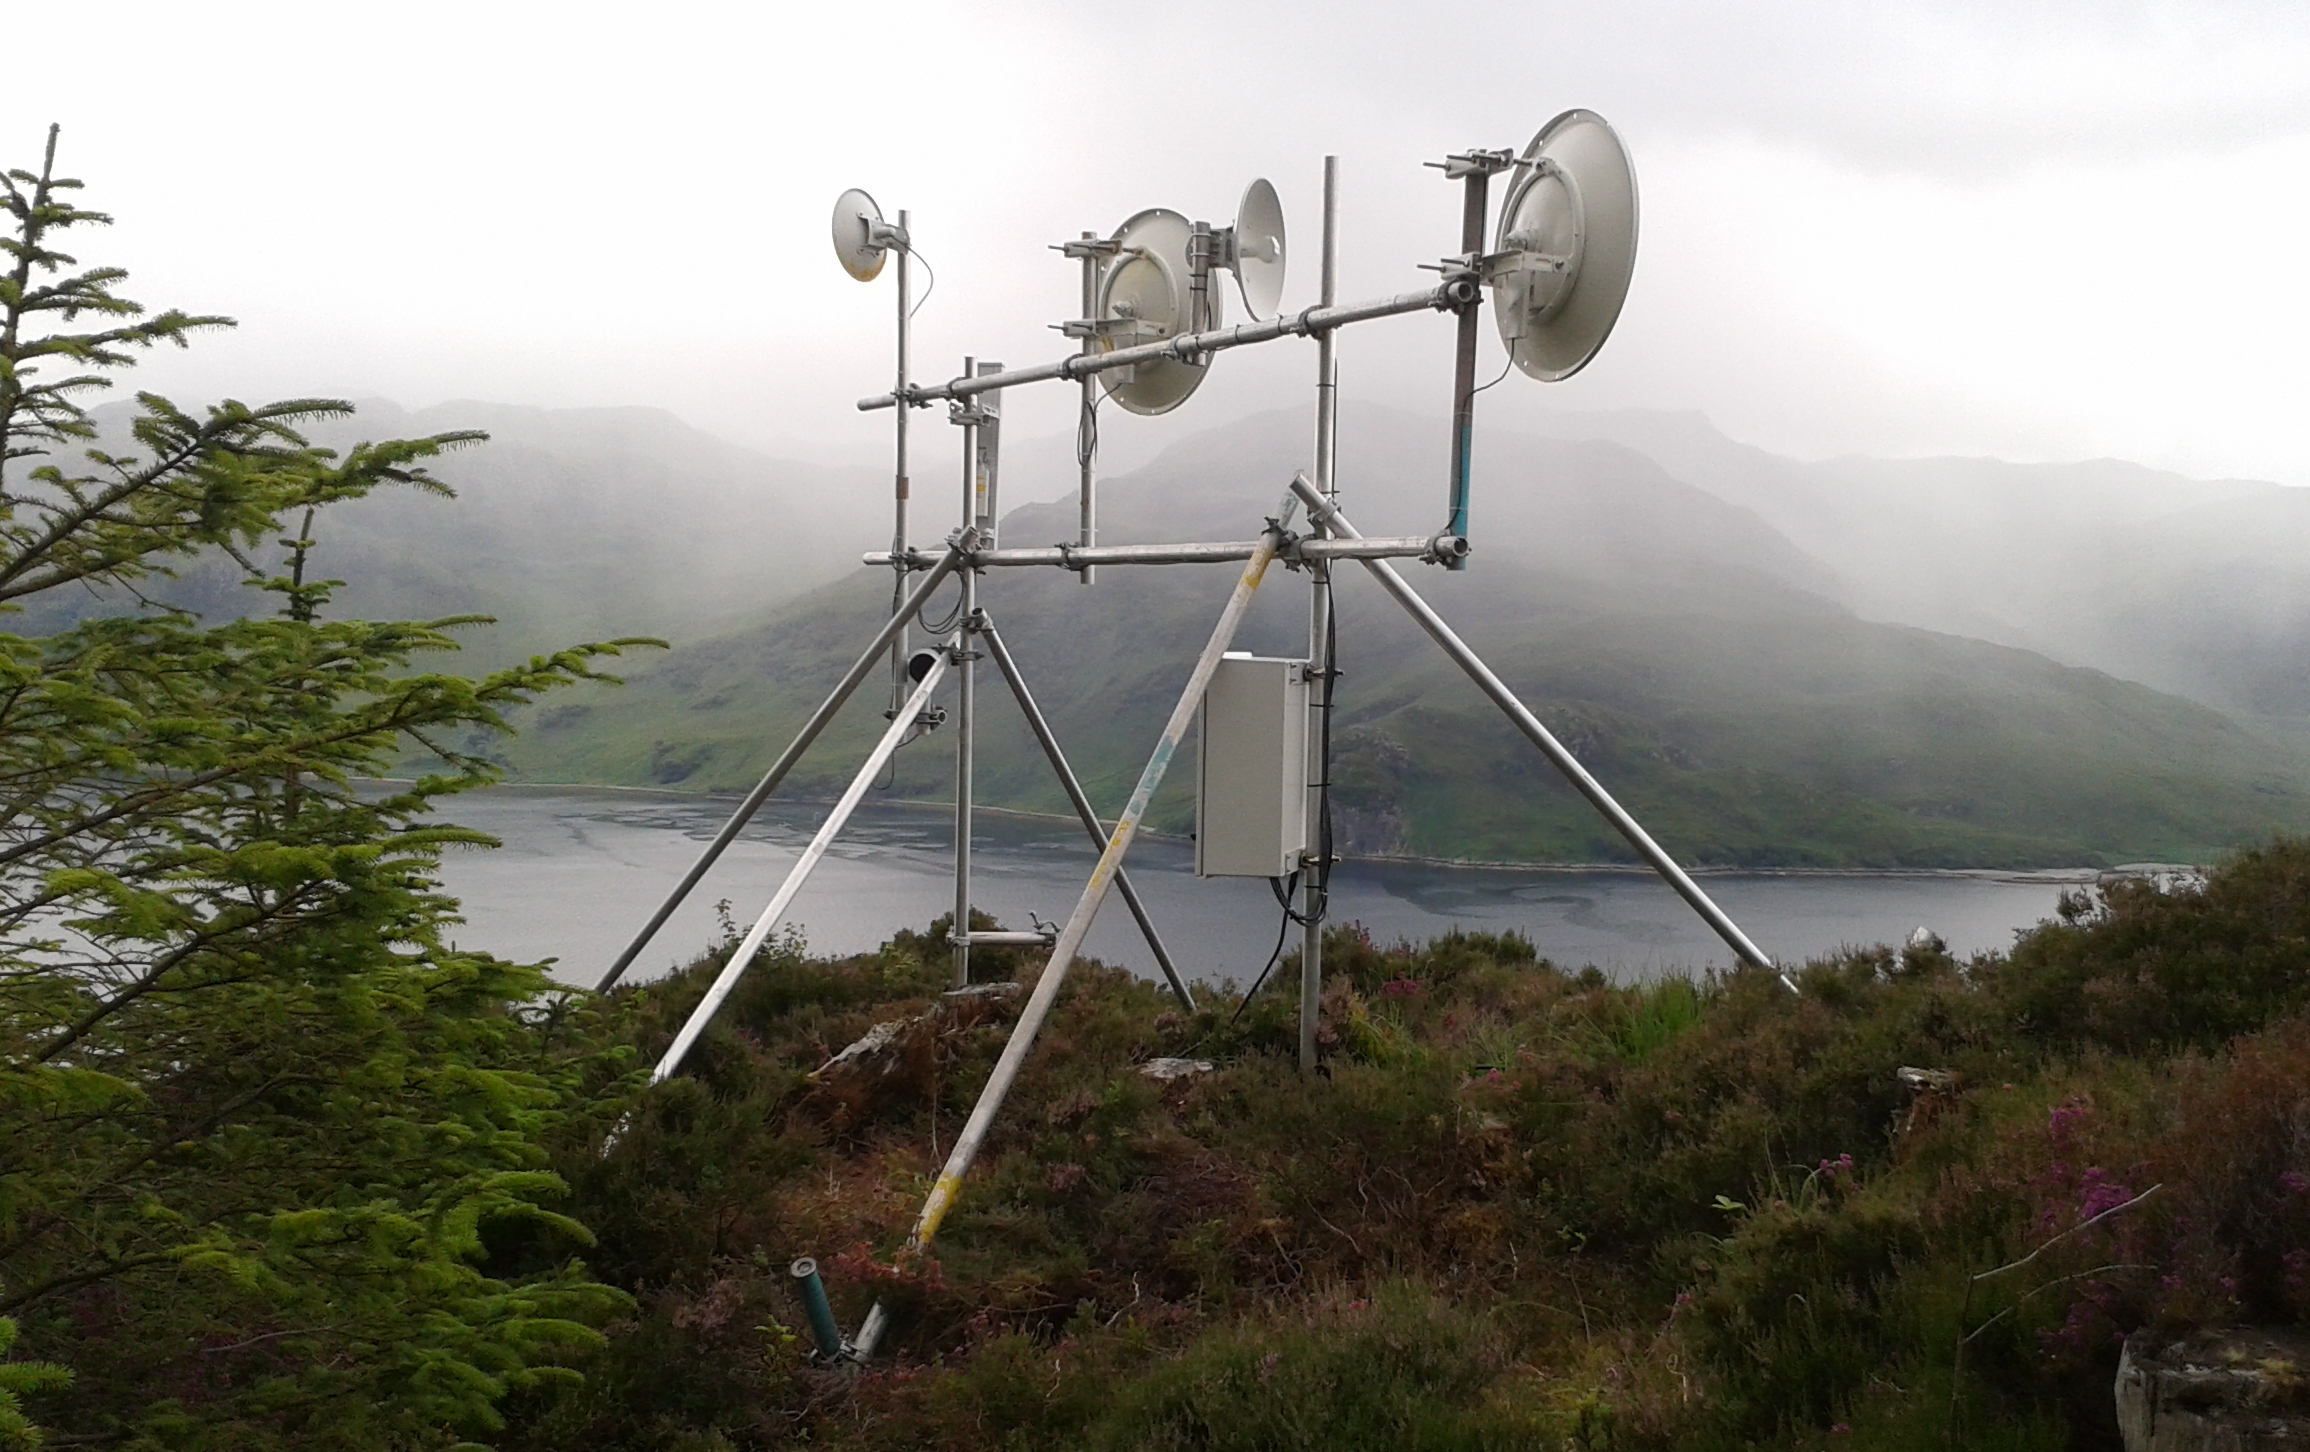
\includegraphics[width=\columnwidth]{figs/mhialairigh-from-behind}
 \caption{A basic relay}
\label{fig:mhialairigh}
\end{figure}

Recently, it has become possible to obtain Ethernet services in two
major towns, but the cost is only reasonable if communities combine
and buy at ``bulk'' prices.  For this one needs two things: an
organization -- a co-operative -- that will act on behalf of the
communities to obtain the economies of scale and a networking
infrastructure

The terrain and the sociology of the Highlands and Island raises some
important issues for both of these.
\begin{itemize}
\item The social communities do not always align well with the
  ``electronic'' communities. It is relatively easy to bounce signals
  back and forth across a loch or glen, but extremely hard to carry
  them over a 1000m high range of mountains. The reasons for this are
  social and economic and sometimes determined by the ways in which
  communities obtain funding.%\footnote{Knoydart is an isolated
    %% peninsula (see Fig.~\ref{fig:whixmap})  of which the North and
    %% West coasts are served by a network based on Loch Hourn and the
    %% South coast is served by Loch Nevis.  Contrast this with the Sleat
    %% peninsula which could, rationally,  be split into three sections,
    %% served by Loch Hourn, Loch Nevis and Eigg, but is run
    %% independently as a single entity with three connections to the
    %% rest of the world.}.
\item Communities structure their networks in various ways, and the
  complexity varies from a single point-to multipoint distribution
  system to a network with six relays  eight or more point-to-point
  links.  In some cases the networks have more than one physical path
  between relays for redundancy.
\item Many adjacent communities have successfully duplicated the local
  access network model. Together they cover a significantly large,
  contiguous geographical area.
\item Communities may temporarily share resources (links or backhaul)
  when appropriate but this is not done in a systematic or organised
  fashion.
\end{itemize}

%% Stimulated in part by developments in the Highlands and Islands,
%% communities in the Scottish Borders South of Edinburgh started to
%% develop similar networks.  While the terrain is also mountainous, the
%% communities are within 40km of Edinburgh where fibre services are
%% available.  However these are only affordable if the communities
%% combine to purchase bandwidth at scale. To this end a community
%% interest company, HUBS, was established whose members are the
%% communities itself.  In addition to backhaul, HUBS provides technical
%% help and other services.  It is anticipated that HUBS will extend its
%% reach to serve the West Coast and achieve further economies of scale,
%% for example in the puchase of transit.


\section{RemIX Architecture} \label{sec:arch} In this section we present the RemIX architecture. We compare RemIX with IXP architectures, and relate those
benefits in the context of remote access networks.

\subsection{Design Requirements}

Our requirements are shaped by three broad goals:
\begin{inparaenum}[(i)]
  \item establish high-quality backhaul to remote regions;
  \item ensure backhaul affordability for small access networks;
  \item allow networks to maintain the autonomy that is
    fundamental to their sustainability.
\end{inparaenum}
%Concretely this means that the
Member networks must be able to connect to one or more transit providers.
Members must also be free to arrange and articulate policies among themselves.
These requirements imply that a \emph{logical} concentration of inter-network
connections is desirable, which suggests a shared switching fabric below the
network layer.

\begin{figure*}
  \subfloat[Traditional IXP]{
    \resizebox{0.45\columnwidth}{!}{
      \begin{tikzpicture}
        \ixboxesA
      \end{tikzpicture}
      \label{fig:ixbA}
    }
  } \hfill
  \subfloat[Modern urban IXP]{
    \resizebox{0.45\columnwidth}{!}{
      \begin{tikzpicture}
        \ixboxesB
      \end{tikzpicture}
      \label{fig:ixbB}
    }
  } \hfill
  \subfloat[RemIX]{
    \resizebox{0.45\columnwidth}{!}{
      \begin{tikzpicture}
        \ixboxesC
      \end{tikzpicture}
      \label{fig:ixbC}
    }
  }
  \caption{Comparison of exchange point models. Notice density.}
  \label{fig:ixb}
\end{figure*}

Networks that are capable of connecting to the same location can do so with an
Ethernet switch. This is the basis for traditional \ac{IXP} design (Fig.~\ref{fig:ixbA}) where member networks connect to a central fabric
with their own router that sits inside the IXP facility. Our remote networks
have no such luxury. In response, we take and distribute the contemporary design
of a multi-site \ac{IXP} (Fig.~\ref{fig:ixbB}). A multi-site \acp{IXP}
presents a single logical fabric to its members, implemented with switches
that are joined by private circuits.
% Since we don't have that luxury, we take the contemporary design of a
% multi-site
% \ac{IXP} as in Figure~\ref{fig:ixbB} and take it to a \emph{maximally
% distributed} extreme---Figure~\ref{fig:ixbC}.

The RemIX architecture that emerges (Fig.~\ref{fig:ixbC})
has no large facility nor physical housing. Instead it is
distributed so that \emph{lightweight} points of presence may be established
where there are as few as two members. Members either colocate their border
routers with the exchange switch, or remotely on the far end of a link, as
circumstances dictate.

These circumstances motivate the lightweight nature of points of presence.
Since the fabric is distributed, fewer networks that will connect from each
site. High port densities are unnecessary. Simultaneously, space and power are
both at a premium. For example, a remote port into RemIX could be housed in a
small cabinet atop a hill, or in space that is donated by a property owner for
this purpose. Equipment is therefore restricted to the small and
power-efficient.


\subsection{RemIX Components}

\subsubsection{Switching Fabric}

The exchange itself must mimic a distributed Ethernet switch. Multiple
Ethernet-like link options include fibre, 802.11 wireless, licensed wireless, fibre, leased pseudo-wires. The switching fabric may be implemented on
top using \acs{BGP}-\acs{VPLS}~\cite{rfc4761} (as we have in
Section~\ref{sec:bgpvpls}),
\acs{BATMAN}~\cite{johnson2008simple}, or
\acs{TRILL}~\cite{perlman2004rbridges} protocols. The salient feature
between them is MAC address learning to establish an Ethernet switch
similar to the \ac{MEF} E-LAN interface
specification~\cite{mef62}.%,mefes}.

\subsubsection{Member \acp{AS}}

Among traditional \acp{IXP} connected networks are encapsulated into
Autonomous Systems (\acp{AS}). Among RemIX member networks, the
policies of the small sized member networks are
%member networks means that the policies are somewhat
different from the Internet's \ac{DFZ}. In particular, member
networks' smaller routers will be neither be capable of storing the
entire Internet routing table, nor are they likely to announce
netblocks large enough to be globally visible.  However, \ac{AS}
\emph{encapsulation} enables networks to retain their internal
structures and methodologies, and to interconnect safely  with
neighbours. Due to the likelihood of collisions use of private
\acp{ASN} is inappropriate for this purpose~\cite{rfc6996}, as are
private IP addresses for the exchange itself~\cite{rfc1918}.

\subsubsection{Exchange Transit}

RemIX members' IP address spaces will be small, and need some entity to
advertise larger netblocks on their behalf. This suggests a specialized transit
provider to mediate between members and the wider Internet. For this reason
RemIX members form a confederation with a transit provider that
presents them collectively to upstream providers and other exchange points. This
is unusual for \acp{IXP}: Rarely are transit relationships implemented with
exchange points. However, this is normal in RemIX, and likely necessary to
function in the intended environment. We note that transit service should be
optional to members, with no requirement to purchase said provider's transit as
a condition for joining the exchange. Also, nothing prevents other such
providers from participating.

\subsubsection{Auxiliary Services}

\acs{BGP} configuration can be a complex. For example, upon
connecting to RemIX, member networks need to be configured to peer amongst
themselves. The complexity quickly increases as session numbers grow with the
square of the number of participants. Instead, \acp{IXP} use
\emph{route-servers} to repeats announcements from one member to all others. A
route reflector keeps the configuration burden to a minimum. Other useful
services such as \acs{NTP} clocks and looking glasses for assistance in
debugging may be offered in addition.

%\subsection{Structural Benefits}

The overall RemIX architecture is motivated by our own needs in Scotland. In
the next section we present our first-phase implementation of RemIX,
alongside remarks on usability and directions for the future.

%\begin{itemize}
%    \item provides default transit to Internet (useful because of IP
%      limits - have to be careful about if/how to raise IP issue)
%    \item BGP solves $n^2$ connects, gives bilateral arrangements
%    \item (in our case) BGP is also the foundation of exchange fabric, i.e.
%      pt2pt circuits that mimic Ethernet
%\end{itemize}


\begin{figure}[h]
  \resizebox{\linewidth}{!}{
    \begin{tikzpicture}
      \whixtopodiagram
    \end{tikzpicture}
  }
  \caption{
  \textbf{Autonomous System topology.} The members of the RemIX in the West
  Highlands, WHIX form a fully connected network where each may communicate
  with another over the exchange without intermediation. HUBS is also present
  and unusually for IXPs will provide Internet transit over the exchange for
  those members that so require. In practice this is most of them. Note as
  well the private interconnection, outwith the exchange, between Skyenet 
  and Hebnet.
  }
\end{figure}

\section{WHIX in Scotland} \label{sec:impl} %\narrative{In this section we describe CIX as implemented by HUBS, a non-profit etc, etc... Then (1) Particulars of implementation in Scotland and how they were dealth with (if they exist). (2) What the current network looks like, and anticipated changes and/or {\bf unanticipated stuffs, lessons learned}. (3) Outcomes as they exist so far.}

In this section we describe our first implementation of RemIX in a series of planned deployments across Scotland. In the West Highlands there
is a cluster of
%%
%% Mull
%% Moidart
%% Small Isles
%% Knoydart
%% Sleat
%% Tegola (experimental, lab)
%% Tegola (production)
%% Glenelg
%% Applecross
%% CMNet
%% Lochiel
%%
11 small community networks. Their spread across $\sim 2000km^2$
%% source -- 100km long by 20km wide
of sea and mountainous islands makes the
construction of an exchange fabric geographically ambitious. Four networks have
a history of interconnecting and sharing network resources, pre-established
relationships that must be respected in our deployment.

Our deployment's location is its namesake, the \ac{WHIX}.
%Both
Logical
and physical layers are described below, with additional lessons and
comments drawn from our experience.

\subsection{West Highland IX at Layer 1}

The physical \ac{WHIX} fabric is overlayed onto a stylized map of the region in
Figure~\ref{fig:whixmap}. The map itself preserves critical geographical
features. Red connected nodes are the connection sites. In a traditional
\ac{IXP} these sites are the Ethernet ports into which subscriber \acp{AS}
plug-in. WHIX sites are connected by wireless radio links in black, and leased
100Mbps or 1Gbps circuits in orange. The areas enclosed with dotted lines
correspond to the service areas reachable from each site.
%%%%% FIGURE %%%%%
\begin{figure*}
  \centering
  \subfloat[Physical topology of \ac{WHIX}.]{
    \resizebox{0.8\columnwidth}{0.3\textheight}{
      \begin{tikzpicture}
        \whixphysicaldiagram
      \end{tikzpicture}
    }
    \label{fig:whixmap}
  }\hfil %\hspace{\columnsep}
  \subfloat[Member connections to \ac{WHIX}]{
    \resizebox{0.8\columnwidth}{0.3\textheight}{
      \begin{tikzpicture}
        \whixmeshdiagram
      \end{tikzpicture}
     }
    \label{fig:phytop}
  }
  \caption{Physical and logical layout of \ac{WHIX}. In
  Figure~\ref{fig:whixmap} the dark lines correspond to radio links
  and the light, curved lines to leased ethernet circuits.
  In Figure~\ref{fig:phytop} the dashed lines
  correspond to internal layer-2 circuits forming \ac{WHIX}
  switching fabric and the solid lines to member connections.}
\end{figure*}

The \ac{WHIX} physical topology in Figure~\ref{fig:whixmap} appears alongside
the member network in Figure~\ref{fig:phytop}. In the latter,
unlabeled red nodes are the \ac{WHIX} points of presence and
correspond with the same set of red nodes in Figure~\ref{fig:whixmap}.
The dashed lines represent the fully connected virtual topology that
implements the exchange E-LAN.

The two places in the region where long-distance ethernet circuits are
available on the mainland are the towns of Mallaig and Kyle of
Lochalsh. Circuits\footnote{\small{At the time of writing, the Mallaig
circuit exists, and that from Kyle is pending.}} from these sites
connect back to the Pulsant datacentre in Edinburgh to facilitate
remote peering --- and indeed the provision of Internet access via the
exchange point.

The radio links are implemented with Ubiquiti Networks equipment,
configured in transparent bridge mode so that they appear as Ethernet from a
functional perspective. The switching fabric itself at each of \ac{WHIX} points
of presence is implemented with Mikrotik routers. This choice was made because
of their moderate port density, low power consumption, low cost, and adequately
featureful \acs{MPLS} implementation. We revisit this choice in the next
section. All equipment is configured to pass Ethernet frames of at least 1600
bytes to provide room for the necessary extra protocol headers for implementing
the E-LAN service.

\subsection{West Highland IX at Layer 2}\label{sec:bgpvpls}

%We emphasize that 
Layer-2 details are \emph{internal} to
\ac{WHIX}, and invisible to members who only see an Ethernet switch. Also, our
implementation decisions are by no means the only possible means of
implementation.

In \ac{WHIX} the requirement for functional equivalence to a \acs{MAC} address
learning Ethernet switch is met using \acs{BGP} signalled
\acs{VPLS}~\cite{rfc4761}. This creates a full set of \acs{LSP} pseudo-wires
between every pair of \ac{WHIX} edge routers.
% It should be emphasised that this section is implementation detail internal to
% \ac{WHIX} and is not visible to the members: all they see is a big Ethernet
% switch. Neither is this the only way to meet the design requirement.
Each \ac{WHIX} router maintains an \acs{OSPF} routing protocol
adjacency with its neighbours and distributes reachability information
for its loopback IP address. All addresses used for this purpose are
private IPv4 addresses~\cite{rfc1918}. This is the basic layer that
ensures reachability throughout the distributed fabric.
%With IP connectivity established,
Non-IP traffic is carried via \acs{LDP}~\cite{rfc5036}
%is used to enable the carriage of non-IP traffic
with \acs{MPLS} labels according to the topology of the underlying \acs{OSPF}
network.

Routers in \ac{WHIX} establish \acs{BGP} peering sessions with routers at
Mallaig and Sabhal M\`{o}r Ostaig that act as route reflectors~\cite{rfc4456}.
Participating routers use route reflectors to exchange reachability information
without requiring a full mesh ($n^2$) of internal peering sessions. The presence
of \acs{BGP} signalling throughout the \ac{WHIX} fabric enables the use of
multi-protocol extensions~\cite{rfc4760}. Routers can use extensions to signal a
desire to form part of the exchange \acs{LAN}.
%% MF- What has a defined target, the extension or the router?
%, which has a defined route target value and in this
The result is a fully meshed \acs{VPLS}, where each router has a virtual bridge
interface that forms part of the exchange \acs{LAN}.

Interfaces can be added to virtual bridges, as needed, to
form part of the exchange. Care must be taken to prevent loops in which members
see the traffic that they originate. This is accomplished with a split-horizon
method~\cite{rfc4762}. Equally, members must be prevented from creating bridge
loops via their own network by employing \acs{MAC} address filter on relevant
ports.

\subsection{West Highland IX at Layer 3+}

Given logical connectivity between all member ports, it remains to
assign IP addresses to their border routers, as well as public
infrastructure such as the router server. As mentioned above the use
of private IP address space for this purpose is undesirable since it
generates risks of collisions with members' own infrastructure.
\ac{WHIX}, and more generally RemIX, is fortunate in this regard: The
design meets the definition of an \ac{IXP}~\cite{ripe451,whixrules},
making it possible to acquire IPv4 and IPv6 address allocations from
RIPE NCC~\cite{ripe649}.

%%%%% FIGURE %%%%%
\begin{figure}[h]
  \resizebox{1.0\linewidth}{!}{
    \begin{tikzpicture}
      \whixtopodiagram
    \end{tikzpicture}
  }
  \caption{
  Autonomous System topology. WHIX members are fully
  connected; communication over the
  exchange needs no intermediation.
  %% Unusually for \acp{IXP} it is
  %% common practice to provide Internet transit over the exchange for
  %% the vast majority of members that require this. Note as well the
  %% private interconnection, outwith the exchange, between Skyenet and
  %% Hebnet. Such private interconnections are typically made as an
  %% optimisation where it is not feasible to do so efficiently over the
  %% exchange.
  }
  \label{fig:l3}
\end{figure}

The full layer-3 \ac{WHIX} topology is shown in Figure~\ref{fig:l3}. At this
stage member network have everything they need. Members can communicate at layer
2. Each has an IP address at layer 3, an autonomous system number for
identification, and their own networks to announce. Bilateral peering
arrangements (an otherwise $n^2$ configuration task) are facilitated by two
route-servers, as before at Mallaig and Sabhal M\`{o}r Ostaig. The route servers
redistribute reachability information, akin to a route-reflector omits its own
\ac{ASN} from the path.

The transit provider, HUBS (see Section~\ref{subsec:hubs}), is also
present at \ac{WHIX} as a member. In addition to public multilateral
peering, it establishes bilateral sessions with members wishing to
announce either a default route or full Internet routing tables. HUBS
forwards those members' announcements upstream and to their peers. In
this way transit, and hence connectivity to the global Internet, is
provided over the exchange.
%\subsection{Usability 'Trade-off'} \label{subsec:use}
%\narrative{Our use of cheap proprietary vs open batman-compatible}


\subsection{Deployment Discussion}

Our experience motivates higher-level comments to further distinguish
RemIX deployments form their larger \ac{IXP} cousins. Flat networks
consisting of a single layer-2 broadcast domain can be plagued by
problems that are difficult to troubleshoot. By its very design RemIX
requires that members be able to communicate directly without
mediation at the IP layer. Like other \acp{IXP} RemIX eliminates a
large class of potential problems by allowing only unicast and
\acs{ARP} traffic on the exchange. Moreover, members must nominate a
specific \acs{MAC} address for their connections, which reduces the
risk of loops and broadcast storms. We also adopt best practices such
as quarantines for new connections while they are evaluated for
correctness.

% Many working network engineers have had the experience of inheriting a flat
% network consisting of a single layer-2 broadcast domain, invariably plagued by
% difficult to troubleshoot problems.

% The architecture is such that the extension of the layer-2 broadcast domain
% extends far enough to meet the design requirements but not so far as to become
% unwieldy.

IP transit in RemIX also deserves to be addressed. Transit
via the exchange, for networks that are not otherwise visible on the Internet,
may evoke notions of conflicting interests that
beset \acp{NAP}. However the similarity is superficial. Here, the transit
provider and exchange operator HUBS \textsc{c.i.c.}, is a cooperative
that exists for the benefit of and is controlled by the members, who
are also members of the \ac{IXP}. As a consequence all parties'
economic interests are aligned.

Finally, \ac{WHIX}' implementation using \acs{BGP}-\acs{VPLS}
to construct the exchange fabric makes it possible to offer auxiliary
point to point pseudo-wire services to its members. This is
useful for those members that have need for making connections internal to their
networks.
% This is as simple as creating a distinct route target
% bridged to two of their ports which results in the establishment of a
% dedicated~\acs{VPLS} instance for them.


\section{Concluding Remarks} \label{sec:conc} %% MF- Moved from 3.3; reads more as final remarks. TBD later.
The features of RemIX described above will be instantly recognisable
to anyone who has participated in a regular \ac{IXP}. This is by
design, as RemIX is an application of a structure that has allowed the
Internet to scale to the rural networking environment. Not only does
encapsulating small community networks in \acp{AS} mean that they can
present a uniform interface to a transit provider but also that it is
possible for them to cooperate and to share resources and yet for each
to retain the ability to operate their own network as they see
fit. This is very important because keeping as much of operations and
maintenance local is the only way they can be sustainable. In turn
this means that the internal details of each network should suit those
doing the work and what they are comfortable with.


\begin{figure}[h]
  \resizebox{\linewidth}{!}{
    \begin{tikzpicture}
      \whixmeshdiagram
    \end{tikzpicture}
  }
\end{figure}

\bibliographystyle{abbrv}
\bibliography{paper_cix}

\end{document}